%% fig_k3threshold.tex   (generated by make_round19.py; do not edit by hand)
%% The threshold t(t+1)/2 of prop:k3powers(ii): the least n with a partition of n having t distinct part sizes, t = 1..21.
\documentclass[tikz,border=8pt]{standalone}
\usepackage{amsmath,amssymb}
\usetikzlibrary{arrows.meta,calc,decorations.pathreplacing}
%% palette.tex -- shared colour definitions for the figures
\definecolor{PInk}{RGB}{26,32,44}
\definecolor{PBlue}{RGB}{37,82,139}
\definecolor{PTeal}{RGB}{23,127,125}
\definecolor{POchre}{RGB}{193,138,44}
\definecolor{PClay}{RGB}{178,74,58}
\definecolor{PSlate}{RGB}{108,122,137}
\definecolor{PViolet}{RGB}{110,86,150}
\definecolor{WBlue}{RGB}{223,234,246}
\definecolor{WTeal}{RGB}{220,238,236}
\definecolor{WOchre}{RGB}{250,240,218}
\definecolor{WClay}{RGB}{247,229,224}
\definecolor{WSlate}{RGB}{238,241,244}
\definecolor{PMag}{RGB}{158,58,110}
\definecolor{PGrass}{RGB}{62,124,66}
\definecolor{PAmber}{RGB}{214,112,38}
\definecolor{PIndigo}{RGB}{58,64,140}
\definecolor{PRule}{RGB}{176,186,197}

%% shared macros so the standalone figures match the paper
\providecommand{\QQ}{\mathbb{Q}}
\providecommand{\ZZ}{\mathbb{Z}}
\providecommand{\RR}{\mathbb{R}}
\providecommand{\CC}{\mathbb{C}}
\providecommand{\PP}{\mathbb{P}}
\providecommand{\Kx}{K^{\times}}
\providecommand{\HW}{W}
\providecommand{\Nm}{\mathrm{N}}
\providecommand{\Hdg}{\mathrm{Hdg}}
\providecommand{\NS}{\mathrm{NS}}
\providecommand{\cA}{\mathcal{A}}
\providecommand{\cD}{\mathcal{D}}
\providecommand{\cF}{\mathcal{F}}
\providecommand{\cP}{\mathcal{P}}
\providecommand{\cO}{\mathcal{O}}
\providecommand{\cQ}{\mathcal{Q}}
\providecommand{\bbar}[1]{\overline{#1}}
\providecommand{\ch}{\operatorname{ch}}
\providecommand{\End}{\mathrm{End}}
\providecommand{\Ext}{\operatorname{Ext}}
\providecommand{\Supp}{\operatorname{Supp}}

\begin{document}
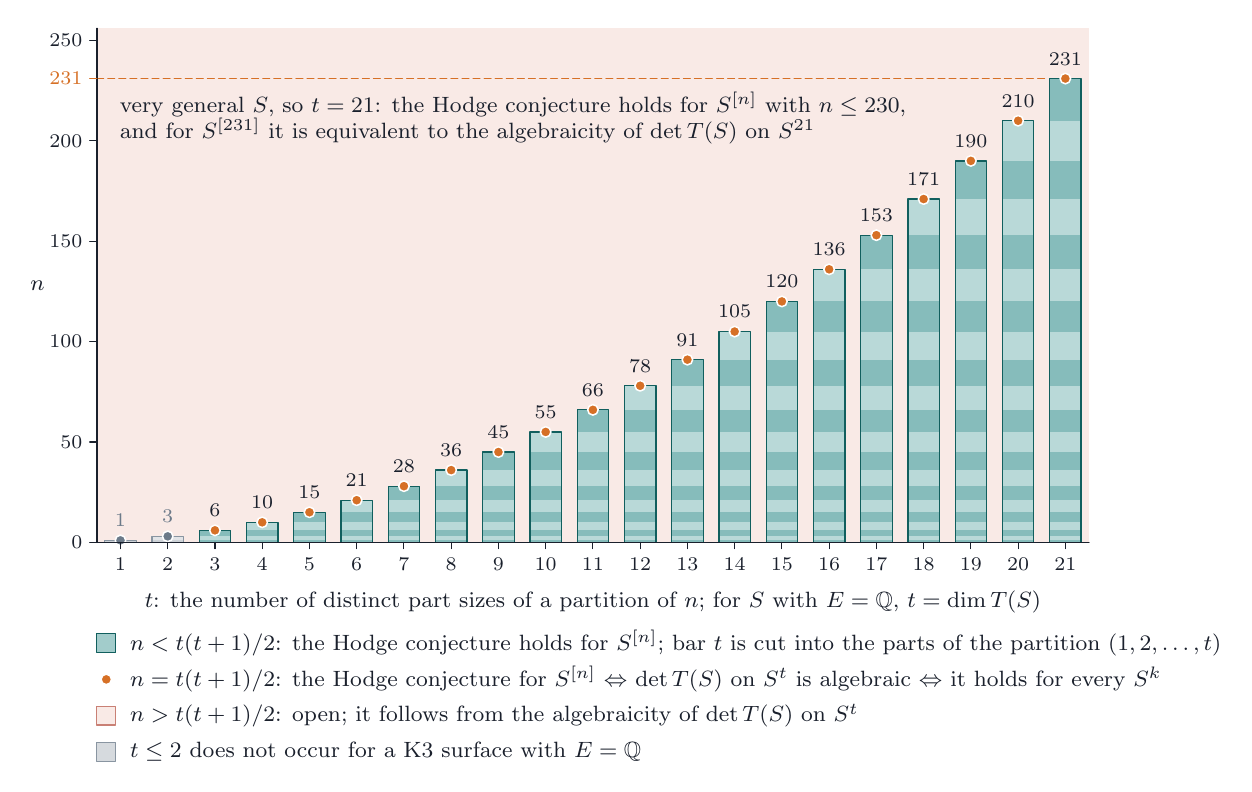
\begin{tikzpicture}[x=1cm,y=1cm,line join=round,line cap=round,
  font=\small,text=PInk,lbl/.style={inner sep=1pt}]
  \path[fill=WClay!80,draw=none] (0.0000,0.0000) rectangle (12.6000,6.5280);
  \path[fill=PSlate!34!white,draw=none] (0.1000,0.0000) rectangle (0.5000,0.0255);
  \path[fill=none,draw=PSlate!80,line width=0.45pt] (0.1000,0.0000) rectangle (0.5000,0.0255);
  \path[fill=PSlate!34!white,draw=none] (0.7000,0.0000) rectangle (1.1000,0.0255);
  \path[fill=PSlate!20!white,draw=none] (0.7000,0.0255) rectangle (1.1000,0.0765);
  \path[fill=none,draw=PSlate!80,line width=0.45pt] (0.7000,0.0000) rectangle (1.1000,0.0765);
  \path[fill=PTeal!52!white,draw=none] (1.3000,0.0000) rectangle (1.7000,0.0255);
  \path[fill=PTeal!30!white,draw=none] (1.3000,0.0255) rectangle (1.7000,0.0765);
  \path[fill=PTeal!52!white,draw=none] (1.3000,0.0765) rectangle (1.7000,0.1530);
  \path[fill=none,draw=PTeal!75!black,line width=0.45pt] (1.3000,0.0000) rectangle (1.7000,0.1530);
  \path[fill=PTeal!52!white,draw=none] (1.9000,0.0000) rectangle (2.3000,0.0255);
  \path[fill=PTeal!30!white,draw=none] (1.9000,0.0255) rectangle (2.3000,0.0765);
  \path[fill=PTeal!52!white,draw=none] (1.9000,0.0765) rectangle (2.3000,0.1530);
  \path[fill=PTeal!30!white,draw=none] (1.9000,0.1530) rectangle (2.3000,0.2550);
  \path[fill=none,draw=PTeal!75!black,line width=0.45pt] (1.9000,0.0000) rectangle (2.3000,0.2550);
  \path[fill=PTeal!52!white,draw=none] (2.5000,0.0000) rectangle (2.9000,0.0255);
  \path[fill=PTeal!30!white,draw=none] (2.5000,0.0255) rectangle (2.9000,0.0765);
  \path[fill=PTeal!52!white,draw=none] (2.5000,0.0765) rectangle (2.9000,0.1530);
  \path[fill=PTeal!30!white,draw=none] (2.5000,0.1530) rectangle (2.9000,0.2550);
  \path[fill=PTeal!52!white,draw=none] (2.5000,0.2550) rectangle (2.9000,0.3825);
  \path[fill=none,draw=PTeal!75!black,line width=0.45pt] (2.5000,0.0000) rectangle (2.9000,0.3825);
  \path[fill=PTeal!52!white,draw=none] (3.1000,0.0000) rectangle (3.5000,0.0255);
  \path[fill=PTeal!30!white,draw=none] (3.1000,0.0255) rectangle (3.5000,0.0765);
  \path[fill=PTeal!52!white,draw=none] (3.1000,0.0765) rectangle (3.5000,0.1530);
  \path[fill=PTeal!30!white,draw=none] (3.1000,0.1530) rectangle (3.5000,0.2550);
  \path[fill=PTeal!52!white,draw=none] (3.1000,0.2550) rectangle (3.5000,0.3825);
  \path[fill=PTeal!30!white,draw=none] (3.1000,0.3825) rectangle (3.5000,0.5355);
  \path[fill=none,draw=PTeal!75!black,line width=0.45pt] (3.1000,0.0000) rectangle (3.5000,0.5355);
  \path[fill=PTeal!52!white,draw=none] (3.7000,0.0000) rectangle (4.1000,0.0255);
  \path[fill=PTeal!30!white,draw=none] (3.7000,0.0255) rectangle (4.1000,0.0765);
  \path[fill=PTeal!52!white,draw=none] (3.7000,0.0765) rectangle (4.1000,0.1530);
  \path[fill=PTeal!30!white,draw=none] (3.7000,0.1530) rectangle (4.1000,0.2550);
  \path[fill=PTeal!52!white,draw=none] (3.7000,0.2550) rectangle (4.1000,0.3825);
  \path[fill=PTeal!30!white,draw=none] (3.7000,0.3825) rectangle (4.1000,0.5355);
  \path[fill=PTeal!52!white,draw=none] (3.7000,0.5355) rectangle (4.1000,0.7140);
  \path[fill=none,draw=PTeal!75!black,line width=0.45pt] (3.7000,0.0000) rectangle (4.1000,0.7140);
  \path[fill=PTeal!52!white,draw=none] (4.3000,0.0000) rectangle (4.7000,0.0255);
  \path[fill=PTeal!30!white,draw=none] (4.3000,0.0255) rectangle (4.7000,0.0765);
  \path[fill=PTeal!52!white,draw=none] (4.3000,0.0765) rectangle (4.7000,0.1530);
  \path[fill=PTeal!30!white,draw=none] (4.3000,0.1530) rectangle (4.7000,0.2550);
  \path[fill=PTeal!52!white,draw=none] (4.3000,0.2550) rectangle (4.7000,0.3825);
  \path[fill=PTeal!30!white,draw=none] (4.3000,0.3825) rectangle (4.7000,0.5355);
  \path[fill=PTeal!52!white,draw=none] (4.3000,0.5355) rectangle (4.7000,0.7140);
  \path[fill=PTeal!30!white,draw=none] (4.3000,0.7140) rectangle (4.7000,0.9180);
  \path[fill=none,draw=PTeal!75!black,line width=0.45pt] (4.3000,0.0000) rectangle (4.7000,0.9180);
  \path[fill=PTeal!52!white,draw=none] (4.9000,0.0000) rectangle (5.3000,0.0255);
  \path[fill=PTeal!30!white,draw=none] (4.9000,0.0255) rectangle (5.3000,0.0765);
  \path[fill=PTeal!52!white,draw=none] (4.9000,0.0765) rectangle (5.3000,0.1530);
  \path[fill=PTeal!30!white,draw=none] (4.9000,0.1530) rectangle (5.3000,0.2550);
  \path[fill=PTeal!52!white,draw=none] (4.9000,0.2550) rectangle (5.3000,0.3825);
  \path[fill=PTeal!30!white,draw=none] (4.9000,0.3825) rectangle (5.3000,0.5355);
  \path[fill=PTeal!52!white,draw=none] (4.9000,0.5355) rectangle (5.3000,0.7140);
  \path[fill=PTeal!30!white,draw=none] (4.9000,0.7140) rectangle (5.3000,0.9180);
  \path[fill=PTeal!52!white,draw=none] (4.9000,0.9180) rectangle (5.3000,1.1475);
  \path[fill=none,draw=PTeal!75!black,line width=0.45pt] (4.9000,0.0000) rectangle (5.3000,1.1475);
  \path[fill=PTeal!52!white,draw=none] (5.5000,0.0000) rectangle (5.9000,0.0255);
  \path[fill=PTeal!30!white,draw=none] (5.5000,0.0255) rectangle (5.9000,0.0765);
  \path[fill=PTeal!52!white,draw=none] (5.5000,0.0765) rectangle (5.9000,0.1530);
  \path[fill=PTeal!30!white,draw=none] (5.5000,0.1530) rectangle (5.9000,0.2550);
  \path[fill=PTeal!52!white,draw=none] (5.5000,0.2550) rectangle (5.9000,0.3825);
  \path[fill=PTeal!30!white,draw=none] (5.5000,0.3825) rectangle (5.9000,0.5355);
  \path[fill=PTeal!52!white,draw=none] (5.5000,0.5355) rectangle (5.9000,0.7140);
  \path[fill=PTeal!30!white,draw=none] (5.5000,0.7140) rectangle (5.9000,0.9180);
  \path[fill=PTeal!52!white,draw=none] (5.5000,0.9180) rectangle (5.9000,1.1475);
  \path[fill=PTeal!30!white,draw=none] (5.5000,1.1475) rectangle (5.9000,1.4025);
  \path[fill=none,draw=PTeal!75!black,line width=0.45pt] (5.5000,0.0000) rectangle (5.9000,1.4025);
  \path[fill=PTeal!52!white,draw=none] (6.1000,0.0000) rectangle (6.5000,0.0255);
  \path[fill=PTeal!30!white,draw=none] (6.1000,0.0255) rectangle (6.5000,0.0765);
  \path[fill=PTeal!52!white,draw=none] (6.1000,0.0765) rectangle (6.5000,0.1530);
  \path[fill=PTeal!30!white,draw=none] (6.1000,0.1530) rectangle (6.5000,0.2550);
  \path[fill=PTeal!52!white,draw=none] (6.1000,0.2550) rectangle (6.5000,0.3825);
  \path[fill=PTeal!30!white,draw=none] (6.1000,0.3825) rectangle (6.5000,0.5355);
  \path[fill=PTeal!52!white,draw=none] (6.1000,0.5355) rectangle (6.5000,0.7140);
  \path[fill=PTeal!30!white,draw=none] (6.1000,0.7140) rectangle (6.5000,0.9180);
  \path[fill=PTeal!52!white,draw=none] (6.1000,0.9180) rectangle (6.5000,1.1475);
  \path[fill=PTeal!30!white,draw=none] (6.1000,1.1475) rectangle (6.5000,1.4025);
  \path[fill=PTeal!52!white,draw=none] (6.1000,1.4025) rectangle (6.5000,1.6830);
  \path[fill=none,draw=PTeal!75!black,line width=0.45pt] (6.1000,0.0000) rectangle (6.5000,1.6830);
  \path[fill=PTeal!52!white,draw=none] (6.7000,0.0000) rectangle (7.1000,0.0255);
  \path[fill=PTeal!30!white,draw=none] (6.7000,0.0255) rectangle (7.1000,0.0765);
  \path[fill=PTeal!52!white,draw=none] (6.7000,0.0765) rectangle (7.1000,0.1530);
  \path[fill=PTeal!30!white,draw=none] (6.7000,0.1530) rectangle (7.1000,0.2550);
  \path[fill=PTeal!52!white,draw=none] (6.7000,0.2550) rectangle (7.1000,0.3825);
  \path[fill=PTeal!30!white,draw=none] (6.7000,0.3825) rectangle (7.1000,0.5355);
  \path[fill=PTeal!52!white,draw=none] (6.7000,0.5355) rectangle (7.1000,0.7140);
  \path[fill=PTeal!30!white,draw=none] (6.7000,0.7140) rectangle (7.1000,0.9180);
  \path[fill=PTeal!52!white,draw=none] (6.7000,0.9180) rectangle (7.1000,1.1475);
  \path[fill=PTeal!30!white,draw=none] (6.7000,1.1475) rectangle (7.1000,1.4025);
  \path[fill=PTeal!52!white,draw=none] (6.7000,1.4025) rectangle (7.1000,1.6830);
  \path[fill=PTeal!30!white,draw=none] (6.7000,1.6830) rectangle (7.1000,1.9890);
  \path[fill=none,draw=PTeal!75!black,line width=0.45pt] (6.7000,0.0000) rectangle (7.1000,1.9890);
  \path[fill=PTeal!52!white,draw=none] (7.3000,0.0000) rectangle (7.7000,0.0255);
  \path[fill=PTeal!30!white,draw=none] (7.3000,0.0255) rectangle (7.7000,0.0765);
  \path[fill=PTeal!52!white,draw=none] (7.3000,0.0765) rectangle (7.7000,0.1530);
  \path[fill=PTeal!30!white,draw=none] (7.3000,0.1530) rectangle (7.7000,0.2550);
  \path[fill=PTeal!52!white,draw=none] (7.3000,0.2550) rectangle (7.7000,0.3825);
  \path[fill=PTeal!30!white,draw=none] (7.3000,0.3825) rectangle (7.7000,0.5355);
  \path[fill=PTeal!52!white,draw=none] (7.3000,0.5355) rectangle (7.7000,0.7140);
  \path[fill=PTeal!30!white,draw=none] (7.3000,0.7140) rectangle (7.7000,0.9180);
  \path[fill=PTeal!52!white,draw=none] (7.3000,0.9180) rectangle (7.7000,1.1475);
  \path[fill=PTeal!30!white,draw=none] (7.3000,1.1475) rectangle (7.7000,1.4025);
  \path[fill=PTeal!52!white,draw=none] (7.3000,1.4025) rectangle (7.7000,1.6830);
  \path[fill=PTeal!30!white,draw=none] (7.3000,1.6830) rectangle (7.7000,1.9890);
  \path[fill=PTeal!52!white,draw=none] (7.3000,1.9890) rectangle (7.7000,2.3205);
  \path[fill=none,draw=PTeal!75!black,line width=0.45pt] (7.3000,0.0000) rectangle (7.7000,2.3205);
  \path[fill=PTeal!52!white,draw=none] (7.9000,0.0000) rectangle (8.3000,0.0255);
  \path[fill=PTeal!30!white,draw=none] (7.9000,0.0255) rectangle (8.3000,0.0765);
  \path[fill=PTeal!52!white,draw=none] (7.9000,0.0765) rectangle (8.3000,0.1530);
  \path[fill=PTeal!30!white,draw=none] (7.9000,0.1530) rectangle (8.3000,0.2550);
  \path[fill=PTeal!52!white,draw=none] (7.9000,0.2550) rectangle (8.3000,0.3825);
  \path[fill=PTeal!30!white,draw=none] (7.9000,0.3825) rectangle (8.3000,0.5355);
  \path[fill=PTeal!52!white,draw=none] (7.9000,0.5355) rectangle (8.3000,0.7140);
  \path[fill=PTeal!30!white,draw=none] (7.9000,0.7140) rectangle (8.3000,0.9180);
  \path[fill=PTeal!52!white,draw=none] (7.9000,0.9180) rectangle (8.3000,1.1475);
  \path[fill=PTeal!30!white,draw=none] (7.9000,1.1475) rectangle (8.3000,1.4025);
  \path[fill=PTeal!52!white,draw=none] (7.9000,1.4025) rectangle (8.3000,1.6830);
  \path[fill=PTeal!30!white,draw=none] (7.9000,1.6830) rectangle (8.3000,1.9890);
  \path[fill=PTeal!52!white,draw=none] (7.9000,1.9890) rectangle (8.3000,2.3205);
  \path[fill=PTeal!30!white,draw=none] (7.9000,2.3205) rectangle (8.3000,2.6775);
  \path[fill=none,draw=PTeal!75!black,line width=0.45pt] (7.9000,0.0000) rectangle (8.3000,2.6775);
  \path[fill=PTeal!52!white,draw=none] (8.5000,0.0000) rectangle (8.9000,0.0255);
  \path[fill=PTeal!30!white,draw=none] (8.5000,0.0255) rectangle (8.9000,0.0765);
  \path[fill=PTeal!52!white,draw=none] (8.5000,0.0765) rectangle (8.9000,0.1530);
  \path[fill=PTeal!30!white,draw=none] (8.5000,0.1530) rectangle (8.9000,0.2550);
  \path[fill=PTeal!52!white,draw=none] (8.5000,0.2550) rectangle (8.9000,0.3825);
  \path[fill=PTeal!30!white,draw=none] (8.5000,0.3825) rectangle (8.9000,0.5355);
  \path[fill=PTeal!52!white,draw=none] (8.5000,0.5355) rectangle (8.9000,0.7140);
  \path[fill=PTeal!30!white,draw=none] (8.5000,0.7140) rectangle (8.9000,0.9180);
  \path[fill=PTeal!52!white,draw=none] (8.5000,0.9180) rectangle (8.9000,1.1475);
  \path[fill=PTeal!30!white,draw=none] (8.5000,1.1475) rectangle (8.9000,1.4025);
  \path[fill=PTeal!52!white,draw=none] (8.5000,1.4025) rectangle (8.9000,1.6830);
  \path[fill=PTeal!30!white,draw=none] (8.5000,1.6830) rectangle (8.9000,1.9890);
  \path[fill=PTeal!52!white,draw=none] (8.5000,1.9890) rectangle (8.9000,2.3205);
  \path[fill=PTeal!30!white,draw=none] (8.5000,2.3205) rectangle (8.9000,2.6775);
  \path[fill=PTeal!52!white,draw=none] (8.5000,2.6775) rectangle (8.9000,3.0600);
  \path[fill=none,draw=PTeal!75!black,line width=0.45pt] (8.5000,0.0000) rectangle (8.9000,3.0600);
  \path[fill=PTeal!52!white,draw=none] (9.1000,0.0000) rectangle (9.5000,0.0255);
  \path[fill=PTeal!30!white,draw=none] (9.1000,0.0255) rectangle (9.5000,0.0765);
  \path[fill=PTeal!52!white,draw=none] (9.1000,0.0765) rectangle (9.5000,0.1530);
  \path[fill=PTeal!30!white,draw=none] (9.1000,0.1530) rectangle (9.5000,0.2550);
  \path[fill=PTeal!52!white,draw=none] (9.1000,0.2550) rectangle (9.5000,0.3825);
  \path[fill=PTeal!30!white,draw=none] (9.1000,0.3825) rectangle (9.5000,0.5355);
  \path[fill=PTeal!52!white,draw=none] (9.1000,0.5355) rectangle (9.5000,0.7140);
  \path[fill=PTeal!30!white,draw=none] (9.1000,0.7140) rectangle (9.5000,0.9180);
  \path[fill=PTeal!52!white,draw=none] (9.1000,0.9180) rectangle (9.5000,1.1475);
  \path[fill=PTeal!30!white,draw=none] (9.1000,1.1475) rectangle (9.5000,1.4025);
  \path[fill=PTeal!52!white,draw=none] (9.1000,1.4025) rectangle (9.5000,1.6830);
  \path[fill=PTeal!30!white,draw=none] (9.1000,1.6830) rectangle (9.5000,1.9890);
  \path[fill=PTeal!52!white,draw=none] (9.1000,1.9890) rectangle (9.5000,2.3205);
  \path[fill=PTeal!30!white,draw=none] (9.1000,2.3205) rectangle (9.5000,2.6775);
  \path[fill=PTeal!52!white,draw=none] (9.1000,2.6775) rectangle (9.5000,3.0600);
  \path[fill=PTeal!30!white,draw=none] (9.1000,3.0600) rectangle (9.5000,3.4680);
  \path[fill=none,draw=PTeal!75!black,line width=0.45pt] (9.1000,0.0000) rectangle (9.5000,3.4680);
  \path[fill=PTeal!52!white,draw=none] (9.7000,0.0000) rectangle (10.1000,0.0255);
  \path[fill=PTeal!30!white,draw=none] (9.7000,0.0255) rectangle (10.1000,0.0765);
  \path[fill=PTeal!52!white,draw=none] (9.7000,0.0765) rectangle (10.1000,0.1530);
  \path[fill=PTeal!30!white,draw=none] (9.7000,0.1530) rectangle (10.1000,0.2550);
  \path[fill=PTeal!52!white,draw=none] (9.7000,0.2550) rectangle (10.1000,0.3825);
  \path[fill=PTeal!30!white,draw=none] (9.7000,0.3825) rectangle (10.1000,0.5355);
  \path[fill=PTeal!52!white,draw=none] (9.7000,0.5355) rectangle (10.1000,0.7140);
  \path[fill=PTeal!30!white,draw=none] (9.7000,0.7140) rectangle (10.1000,0.9180);
  \path[fill=PTeal!52!white,draw=none] (9.7000,0.9180) rectangle (10.1000,1.1475);
  \path[fill=PTeal!30!white,draw=none] (9.7000,1.1475) rectangle (10.1000,1.4025);
  \path[fill=PTeal!52!white,draw=none] (9.7000,1.4025) rectangle (10.1000,1.6830);
  \path[fill=PTeal!30!white,draw=none] (9.7000,1.6830) rectangle (10.1000,1.9890);
  \path[fill=PTeal!52!white,draw=none] (9.7000,1.9890) rectangle (10.1000,2.3205);
  \path[fill=PTeal!30!white,draw=none] (9.7000,2.3205) rectangle (10.1000,2.6775);
  \path[fill=PTeal!52!white,draw=none] (9.7000,2.6775) rectangle (10.1000,3.0600);
  \path[fill=PTeal!30!white,draw=none] (9.7000,3.0600) rectangle (10.1000,3.4680);
  \path[fill=PTeal!52!white,draw=none] (9.7000,3.4680) rectangle (10.1000,3.9015);
  \path[fill=none,draw=PTeal!75!black,line width=0.45pt] (9.7000,0.0000) rectangle (10.1000,3.9015);
  \path[fill=PTeal!52!white,draw=none] (10.3000,0.0000) rectangle (10.7000,0.0255);
  \path[fill=PTeal!30!white,draw=none] (10.3000,0.0255) rectangle (10.7000,0.0765);
  \path[fill=PTeal!52!white,draw=none] (10.3000,0.0765) rectangle (10.7000,0.1530);
  \path[fill=PTeal!30!white,draw=none] (10.3000,0.1530) rectangle (10.7000,0.2550);
  \path[fill=PTeal!52!white,draw=none] (10.3000,0.2550) rectangle (10.7000,0.3825);
  \path[fill=PTeal!30!white,draw=none] (10.3000,0.3825) rectangle (10.7000,0.5355);
  \path[fill=PTeal!52!white,draw=none] (10.3000,0.5355) rectangle (10.7000,0.7140);
  \path[fill=PTeal!30!white,draw=none] (10.3000,0.7140) rectangle (10.7000,0.9180);
  \path[fill=PTeal!52!white,draw=none] (10.3000,0.9180) rectangle (10.7000,1.1475);
  \path[fill=PTeal!30!white,draw=none] (10.3000,1.1475) rectangle (10.7000,1.4025);
  \path[fill=PTeal!52!white,draw=none] (10.3000,1.4025) rectangle (10.7000,1.6830);
  \path[fill=PTeal!30!white,draw=none] (10.3000,1.6830) rectangle (10.7000,1.9890);
  \path[fill=PTeal!52!white,draw=none] (10.3000,1.9890) rectangle (10.7000,2.3205);
  \path[fill=PTeal!30!white,draw=none] (10.3000,2.3205) rectangle (10.7000,2.6775);
  \path[fill=PTeal!52!white,draw=none] (10.3000,2.6775) rectangle (10.7000,3.0600);
  \path[fill=PTeal!30!white,draw=none] (10.3000,3.0600) rectangle (10.7000,3.4680);
  \path[fill=PTeal!52!white,draw=none] (10.3000,3.4680) rectangle (10.7000,3.9015);
  \path[fill=PTeal!30!white,draw=none] (10.3000,3.9015) rectangle (10.7000,4.3605);
  \path[fill=none,draw=PTeal!75!black,line width=0.45pt] (10.3000,0.0000) rectangle (10.7000,4.3605);
  \path[fill=PTeal!52!white,draw=none] (10.9000,0.0000) rectangle (11.3000,0.0255);
  \path[fill=PTeal!30!white,draw=none] (10.9000,0.0255) rectangle (11.3000,0.0765);
  \path[fill=PTeal!52!white,draw=none] (10.9000,0.0765) rectangle (11.3000,0.1530);
  \path[fill=PTeal!30!white,draw=none] (10.9000,0.1530) rectangle (11.3000,0.2550);
  \path[fill=PTeal!52!white,draw=none] (10.9000,0.2550) rectangle (11.3000,0.3825);
  \path[fill=PTeal!30!white,draw=none] (10.9000,0.3825) rectangle (11.3000,0.5355);
  \path[fill=PTeal!52!white,draw=none] (10.9000,0.5355) rectangle (11.3000,0.7140);
  \path[fill=PTeal!30!white,draw=none] (10.9000,0.7140) rectangle (11.3000,0.9180);
  \path[fill=PTeal!52!white,draw=none] (10.9000,0.9180) rectangle (11.3000,1.1475);
  \path[fill=PTeal!30!white,draw=none] (10.9000,1.1475) rectangle (11.3000,1.4025);
  \path[fill=PTeal!52!white,draw=none] (10.9000,1.4025) rectangle (11.3000,1.6830);
  \path[fill=PTeal!30!white,draw=none] (10.9000,1.6830) rectangle (11.3000,1.9890);
  \path[fill=PTeal!52!white,draw=none] (10.9000,1.9890) rectangle (11.3000,2.3205);
  \path[fill=PTeal!30!white,draw=none] (10.9000,2.3205) rectangle (11.3000,2.6775);
  \path[fill=PTeal!52!white,draw=none] (10.9000,2.6775) rectangle (11.3000,3.0600);
  \path[fill=PTeal!30!white,draw=none] (10.9000,3.0600) rectangle (11.3000,3.4680);
  \path[fill=PTeal!52!white,draw=none] (10.9000,3.4680) rectangle (11.3000,3.9015);
  \path[fill=PTeal!30!white,draw=none] (10.9000,3.9015) rectangle (11.3000,4.3605);
  \path[fill=PTeal!52!white,draw=none] (10.9000,4.3605) rectangle (11.3000,4.8450);
  \path[fill=none,draw=PTeal!75!black,line width=0.45pt] (10.9000,0.0000) rectangle (11.3000,4.8450);
  \path[fill=PTeal!52!white,draw=none] (11.5000,0.0000) rectangle (11.9000,0.0255);
  \path[fill=PTeal!30!white,draw=none] (11.5000,0.0255) rectangle (11.9000,0.0765);
  \path[fill=PTeal!52!white,draw=none] (11.5000,0.0765) rectangle (11.9000,0.1530);
  \path[fill=PTeal!30!white,draw=none] (11.5000,0.1530) rectangle (11.9000,0.2550);
  \path[fill=PTeal!52!white,draw=none] (11.5000,0.2550) rectangle (11.9000,0.3825);
  \path[fill=PTeal!30!white,draw=none] (11.5000,0.3825) rectangle (11.9000,0.5355);
  \path[fill=PTeal!52!white,draw=none] (11.5000,0.5355) rectangle (11.9000,0.7140);
  \path[fill=PTeal!30!white,draw=none] (11.5000,0.7140) rectangle (11.9000,0.9180);
  \path[fill=PTeal!52!white,draw=none] (11.5000,0.9180) rectangle (11.9000,1.1475);
  \path[fill=PTeal!30!white,draw=none] (11.5000,1.1475) rectangle (11.9000,1.4025);
  \path[fill=PTeal!52!white,draw=none] (11.5000,1.4025) rectangle (11.9000,1.6830);
  \path[fill=PTeal!30!white,draw=none] (11.5000,1.6830) rectangle (11.9000,1.9890);
  \path[fill=PTeal!52!white,draw=none] (11.5000,1.9890) rectangle (11.9000,2.3205);
  \path[fill=PTeal!30!white,draw=none] (11.5000,2.3205) rectangle (11.9000,2.6775);
  \path[fill=PTeal!52!white,draw=none] (11.5000,2.6775) rectangle (11.9000,3.0600);
  \path[fill=PTeal!30!white,draw=none] (11.5000,3.0600) rectangle (11.9000,3.4680);
  \path[fill=PTeal!52!white,draw=none] (11.5000,3.4680) rectangle (11.9000,3.9015);
  \path[fill=PTeal!30!white,draw=none] (11.5000,3.9015) rectangle (11.9000,4.3605);
  \path[fill=PTeal!52!white,draw=none] (11.5000,4.3605) rectangle (11.9000,4.8450);
  \path[fill=PTeal!30!white,draw=none] (11.5000,4.8450) rectangle (11.9000,5.3550);
  \path[fill=none,draw=PTeal!75!black,line width=0.45pt] (11.5000,0.0000) rectangle (11.9000,5.3550);
  \path[fill=PTeal!52!white,draw=none] (12.1000,0.0000) rectangle (12.5000,0.0255);
  \path[fill=PTeal!30!white,draw=none] (12.1000,0.0255) rectangle (12.5000,0.0765);
  \path[fill=PTeal!52!white,draw=none] (12.1000,0.0765) rectangle (12.5000,0.1530);
  \path[fill=PTeal!30!white,draw=none] (12.1000,0.1530) rectangle (12.5000,0.2550);
  \path[fill=PTeal!52!white,draw=none] (12.1000,0.2550) rectangle (12.5000,0.3825);
  \path[fill=PTeal!30!white,draw=none] (12.1000,0.3825) rectangle (12.5000,0.5355);
  \path[fill=PTeal!52!white,draw=none] (12.1000,0.5355) rectangle (12.5000,0.7140);
  \path[fill=PTeal!30!white,draw=none] (12.1000,0.7140) rectangle (12.5000,0.9180);
  \path[fill=PTeal!52!white,draw=none] (12.1000,0.9180) rectangle (12.5000,1.1475);
  \path[fill=PTeal!30!white,draw=none] (12.1000,1.1475) rectangle (12.5000,1.4025);
  \path[fill=PTeal!52!white,draw=none] (12.1000,1.4025) rectangle (12.5000,1.6830);
  \path[fill=PTeal!30!white,draw=none] (12.1000,1.6830) rectangle (12.5000,1.9890);
  \path[fill=PTeal!52!white,draw=none] (12.1000,1.9890) rectangle (12.5000,2.3205);
  \path[fill=PTeal!30!white,draw=none] (12.1000,2.3205) rectangle (12.5000,2.6775);
  \path[fill=PTeal!52!white,draw=none] (12.1000,2.6775) rectangle (12.5000,3.0600);
  \path[fill=PTeal!30!white,draw=none] (12.1000,3.0600) rectangle (12.5000,3.4680);
  \path[fill=PTeal!52!white,draw=none] (12.1000,3.4680) rectangle (12.5000,3.9015);
  \path[fill=PTeal!30!white,draw=none] (12.1000,3.9015) rectangle (12.5000,4.3605);
  \path[fill=PTeal!52!white,draw=none] (12.1000,4.3605) rectangle (12.5000,4.8450);
  \path[fill=PTeal!30!white,draw=none] (12.1000,4.8450) rectangle (12.5000,5.3550);
  \path[fill=PTeal!52!white,draw=none] (12.1000,5.3550) rectangle (12.5000,5.8905);
  \path[fill=none,draw=PTeal!75!black,line width=0.45pt] (12.1000,0.0000) rectangle (12.5000,5.8905);
  \path[fill=PSlate,draw=white,line width=0.55pt] (0.3000,0.0255) circle (1.90pt);
  \path[fill=PSlate,draw=white,line width=0.55pt] (0.9000,0.0765) circle (1.90pt);
  \path[fill=PAmber,draw=white,line width=0.55pt] (1.5000,0.1530) circle (1.90pt);
  \path[fill=PAmber,draw=white,line width=0.55pt] (2.1000,0.2550) circle (1.90pt);
  \path[fill=PAmber,draw=white,line width=0.55pt] (2.7000,0.3825) circle (1.90pt);
  \path[fill=PAmber,draw=white,line width=0.55pt] (3.3000,0.5355) circle (1.90pt);
  \path[fill=PAmber,draw=white,line width=0.55pt] (3.9000,0.7140) circle (1.90pt);
  \path[fill=PAmber,draw=white,line width=0.55pt] (4.5000,0.9180) circle (1.90pt);
  \path[fill=PAmber,draw=white,line width=0.55pt] (5.1000,1.1475) circle (1.90pt);
  \path[fill=PAmber,draw=white,line width=0.55pt] (5.7000,1.4025) circle (1.90pt);
  \path[fill=PAmber,draw=white,line width=0.55pt] (6.3000,1.6830) circle (1.90pt);
  \path[fill=PAmber,draw=white,line width=0.55pt] (6.9000,1.9890) circle (1.90pt);
  \path[fill=PAmber,draw=white,line width=0.55pt] (7.5000,2.3205) circle (1.90pt);
  \path[fill=PAmber,draw=white,line width=0.55pt] (8.1000,2.6775) circle (1.90pt);
  \path[fill=PAmber,draw=white,line width=0.55pt] (8.7000,3.0600) circle (1.90pt);
  \path[fill=PAmber,draw=white,line width=0.55pt] (9.3000,3.4680) circle (1.90pt);
  \path[fill=PAmber,draw=white,line width=0.55pt] (9.9000,3.9015) circle (1.90pt);
  \path[fill=PAmber,draw=white,line width=0.55pt] (10.5000,4.3605) circle (1.90pt);
  \path[fill=PAmber,draw=white,line width=0.55pt] (11.1000,4.8450) circle (1.90pt);
  \path[fill=PAmber,draw=white,line width=0.55pt] (11.7000,5.3550) circle (1.90pt);
  \path[fill=PAmber,draw=white,line width=0.55pt] (12.3000,5.8905) circle (1.90pt);
  \draw[PAmber,line width=0.55pt,dash pattern=on 2.4pt off 1.6pt] (0.0000,5.8905) -- (12.0400,5.8905);
  \draw[PInk,line width=0.5pt] (0.0000,0.0000) -- (12.6000,0.0000);
  \draw[PInk,line width=0.5pt] (0.0000,0.0000) -- (0.0000,6.5280);
  \draw[PInk,line width=0.4pt] (-0.0900,0.0000) -- (0.0000,0.0000);
  \draw[PInk,line width=0.4pt] (-0.0900,1.2750) -- (0.0000,1.2750);
  \draw[PInk,line width=0.4pt] (-0.0900,2.5500) -- (0.0000,2.5500);
  \draw[PInk,line width=0.4pt] (-0.0900,3.8250) -- (0.0000,3.8250);
  \draw[PInk,line width=0.4pt] (-0.0900,5.1000) -- (0.0000,5.1000);
  \draw[PInk,line width=0.4pt] (-0.0900,6.3750) -- (0.0000,6.3750);
  \draw[PAmber,line width=0.5pt] (-0.0900,5.8905) -- (0.0000,5.8905);
  \draw[PInk,line width=0.4pt] (0.3000,0.0000) -- (0.3000,-0.0800);
  \draw[PInk,line width=0.4pt] (0.9000,0.0000) -- (0.9000,-0.0800);
  \draw[PInk,line width=0.4pt] (1.5000,0.0000) -- (1.5000,-0.0800);
  \draw[PInk,line width=0.4pt] (2.1000,0.0000) -- (2.1000,-0.0800);
  \draw[PInk,line width=0.4pt] (2.7000,0.0000) -- (2.7000,-0.0800);
  \draw[PInk,line width=0.4pt] (3.3000,0.0000) -- (3.3000,-0.0800);
  \draw[PInk,line width=0.4pt] (3.9000,0.0000) -- (3.9000,-0.0800);
  \draw[PInk,line width=0.4pt] (4.5000,0.0000) -- (4.5000,-0.0800);
  \draw[PInk,line width=0.4pt] (5.1000,0.0000) -- (5.1000,-0.0800);
  \draw[PInk,line width=0.4pt] (5.7000,0.0000) -- (5.7000,-0.0800);
  \draw[PInk,line width=0.4pt] (6.3000,0.0000) -- (6.3000,-0.0800);
  \draw[PInk,line width=0.4pt] (6.9000,0.0000) -- (6.9000,-0.0800);
  \draw[PInk,line width=0.4pt] (7.5000,0.0000) -- (7.5000,-0.0800);
  \draw[PInk,line width=0.4pt] (8.1000,0.0000) -- (8.1000,-0.0800);
  \draw[PInk,line width=0.4pt] (8.7000,0.0000) -- (8.7000,-0.0800);
  \draw[PInk,line width=0.4pt] (9.3000,0.0000) -- (9.3000,-0.0800);
  \draw[PInk,line width=0.4pt] (9.9000,0.0000) -- (9.9000,-0.0800);
  \draw[PInk,line width=0.4pt] (10.5000,0.0000) -- (10.5000,-0.0800);
  \draw[PInk,line width=0.4pt] (11.1000,0.0000) -- (11.1000,-0.0800);
  \draw[PInk,line width=0.4pt] (11.7000,0.0000) -- (11.7000,-0.0800);
  \draw[PInk,line width=0.4pt] (12.3000,0.0000) -- (12.3000,-0.0800);
  \path[fill=PTeal!40!white,draw=PTeal!75!black,line width=0.45pt] (0.0000,-1.4000) rectangle (0.2400,-1.1600);
  \path[fill=PAmber,draw=white,line width=0.55pt] (0.1200,-1.7400) circle (1.90pt);
  \path[fill=WClay!80,draw=PClay!70,line width=0.45pt] (0.0000,-2.3200) rectangle (0.2400,-2.0800);
  \path[fill=PSlate!28!white,draw=PSlate!80,line width=0.45pt] (0.0000,-2.7800) rectangle (0.2400,-2.5400);
  \node[lbl,anchor=south,text=PSlate,font=\scriptsize] at (0.3000,0.1555) {$1$};
  \node[lbl,anchor=south,text=PSlate,font=\scriptsize] at (0.9000,0.2065) {$3$};
  \node[lbl,anchor=south,text=PInk,font=\scriptsize] at (1.5000,0.2830) {$6$};
  \node[lbl,anchor=south,text=PInk,font=\scriptsize] at (2.1000,0.3850) {$10$};
  \node[lbl,anchor=south,text=PInk,font=\scriptsize] at (2.7000,0.5125) {$15$};
  \node[lbl,anchor=south,text=PInk,font=\scriptsize] at (3.3000,0.6655) {$21$};
  \node[lbl,anchor=south,text=PInk,font=\scriptsize] at (3.9000,0.8440) {$28$};
  \node[lbl,anchor=south,text=PInk,font=\scriptsize] at (4.5000,1.0480) {$36$};
  \node[lbl,anchor=south,text=PInk,font=\scriptsize] at (5.1000,1.2775) {$45$};
  \node[lbl,anchor=south,text=PInk,font=\scriptsize] at (5.7000,1.5325) {$55$};
  \node[lbl,anchor=south,text=PInk,font=\scriptsize] at (6.3000,1.8130) {$66$};
  \node[lbl,anchor=south,text=PInk,font=\scriptsize] at (6.9000,2.1190) {$78$};
  \node[lbl,anchor=south,text=PInk,font=\scriptsize] at (7.5000,2.4505) {$91$};
  \node[lbl,anchor=south,text=PInk,font=\scriptsize] at (8.1000,2.8075) {$105$};
  \node[lbl,anchor=south,text=PInk,font=\scriptsize] at (8.7000,3.1900) {$120$};
  \node[lbl,anchor=south,text=PInk,font=\scriptsize] at (9.3000,3.5980) {$136$};
  \node[lbl,anchor=south,text=PInk,font=\scriptsize] at (9.9000,4.0315) {$153$};
  \node[lbl,anchor=south,text=PInk,font=\scriptsize] at (10.5000,4.4905) {$171$};
  \node[lbl,anchor=south,text=PInk,font=\scriptsize] at (11.1000,4.9750) {$190$};
  \node[lbl,anchor=south,text=PInk,font=\scriptsize] at (11.7000,5.4850) {$210$};
  \node[lbl,anchor=south,text=PInk,font=\scriptsize] at (12.3000,6.0205) {$231$};
  \node[lbl,anchor=west,text=PInk,font=\footnotesize,align=left] at (0.2500,5.3875) {very general $S$, so $t=21$: the Hodge conjecture holds for $S^{[n]}$ with $n\le230$,\\and for $S^{[231]}$ it is equivalent to the algebraicity of $\det T(S)$ on $S^{21}$};
  \node[lbl,anchor=east,text=PInk,font=\scriptsize] at (-0.1400,0.0000) {$0$};
  \node[lbl,anchor=east,text=PInk,font=\scriptsize] at (-0.1400,1.2750) {$50$};
  \node[lbl,anchor=east,text=PInk,font=\scriptsize] at (-0.1400,2.5500) {$100$};
  \node[lbl,anchor=east,text=PInk,font=\scriptsize] at (-0.1400,3.8250) {$150$};
  \node[lbl,anchor=east,text=PInk,font=\scriptsize] at (-0.1400,5.1000) {$200$};
  \node[lbl,anchor=east,text=PInk,font=\scriptsize] at (-0.1400,6.3750) {$250$};
  \node[lbl,anchor=east,text=PAmber,font=\scriptsize] at (-0.1400,5.8905) {$231$};
  \node[lbl,anchor=north,text=PInk,font=\scriptsize] at (0.3000,-0.1600) {$1$};
  \node[lbl,anchor=north,text=PInk,font=\scriptsize] at (0.9000,-0.1600) {$2$};
  \node[lbl,anchor=north,text=PInk,font=\scriptsize] at (1.5000,-0.1600) {$3$};
  \node[lbl,anchor=north,text=PInk,font=\scriptsize] at (2.1000,-0.1600) {$4$};
  \node[lbl,anchor=north,text=PInk,font=\scriptsize] at (2.7000,-0.1600) {$5$};
  \node[lbl,anchor=north,text=PInk,font=\scriptsize] at (3.3000,-0.1600) {$6$};
  \node[lbl,anchor=north,text=PInk,font=\scriptsize] at (3.9000,-0.1600) {$7$};
  \node[lbl,anchor=north,text=PInk,font=\scriptsize] at (4.5000,-0.1600) {$8$};
  \node[lbl,anchor=north,text=PInk,font=\scriptsize] at (5.1000,-0.1600) {$9$};
  \node[lbl,anchor=north,text=PInk,font=\scriptsize] at (5.7000,-0.1600) {$10$};
  \node[lbl,anchor=north,text=PInk,font=\scriptsize] at (6.3000,-0.1600) {$11$};
  \node[lbl,anchor=north,text=PInk,font=\scriptsize] at (6.9000,-0.1600) {$12$};
  \node[lbl,anchor=north,text=PInk,font=\scriptsize] at (7.5000,-0.1600) {$13$};
  \node[lbl,anchor=north,text=PInk,font=\scriptsize] at (8.1000,-0.1600) {$14$};
  \node[lbl,anchor=north,text=PInk,font=\scriptsize] at (8.7000,-0.1600) {$15$};
  \node[lbl,anchor=north,text=PInk,font=\scriptsize] at (9.3000,-0.1600) {$16$};
  \node[lbl,anchor=north,text=PInk,font=\scriptsize] at (9.9000,-0.1600) {$17$};
  \node[lbl,anchor=north,text=PInk,font=\scriptsize] at (10.5000,-0.1600) {$18$};
  \node[lbl,anchor=north,text=PInk,font=\scriptsize] at (11.1000,-0.1600) {$19$};
  \node[lbl,anchor=north,text=PInk,font=\scriptsize] at (11.7000,-0.1600) {$20$};
  \node[lbl,anchor=north,text=PInk,font=\scriptsize] at (12.3000,-0.1600) {$21$};
  \node[lbl,anchor=north,text=PInk,font=\footnotesize] at (6.3000,-0.5800) {$t$: the number of distinct part sizes of a partition of $n$; for $S$ with $E=\QQ$, $t=\dim T(S)$};
  \node[lbl,anchor=east,text=PInk,font=\footnotesize] at (-0.6200,3.2640) {$n$};
  \node[lbl,anchor=west,text=PInk,font=\footnotesize] at (0.3800,-1.2800) {$n<t(t+1)/2$: the Hodge conjecture holds for $S^{[n]}$; bar $t$ is cut into the parts of the partition $(1,2,\dots,t)$};
  \node[lbl,anchor=west,text=PInk,font=\footnotesize] at (0.3800,-1.7400) {$n=t(t+1)/2$: the Hodge conjecture for $S^{[n]}$ $\Leftrightarrow$ $\det T(S)$ on $S^{t}$ is algebraic $\Leftrightarrow$ it holds for every $S^{k}$};
  \node[lbl,anchor=west,text=PInk,font=\footnotesize] at (0.3800,-2.2000) {$n>t(t+1)/2$: open; it follows from the algebraicity of $\det T(S)$ on $S^{t}$};
  \node[lbl,anchor=west,text=PInk,font=\footnotesize] at (0.3800,-2.6600) {$t\le2$ does not occur for a K3 surface with $E=\QQ$};
\end{tikzpicture}
\end{document}
